\documentclass[letterpaper, 12pt]{article}
\usepackage[margin=1in]{geometry}
\usepackage{amsmath}
\usepackage{pgfplots}
\usepackage{listings}
\usepackage{graphicx}
\pgfplotsset{width=15cm,compat=1.9} \newcommand{\todo}[1]{{\emph{\color{red}#1}}}
\title{WIP: The Optimization of Alcoholism under a Hypothetical Bartering System}
\author{Kevin Palani and Kevin Zheng}
\begin{document}
\maketitle
\tableofcontents
\section{Introduction to the hypothetical bartering system}
\par You have \$10, and a beer is 2\$.
Very quickly you can see that if you spend all 10\$, you will get 5 beers.
Once you've drunken the 5 beers, you are left with 5 beer bottles and 5 caps.
The store owner strikes you a deal.
If you give him two empty bottles or four bottle caps, he'll give you a new bottle of beer.
He is also kind enough to let you drink before you pay.
How many drinks you can get?
\section{Modeling amount of caps and bottles}
\subsection{Vector representation of caps and bottles}
\[
    \begin{bmatrix}
        a\\
        b\\
        1\\
    \end{bmatrix}
\]
\par Will be the vector that represents the bottles and caps such that $a$ is the amount of bottles, and $b$ is the amount of caps.
The $1$ is a homogenization of the vector.
\subsection{Matrix representation of the bartering system}
\par If we can spend two empty bottles and receive a full drink, that is equivalent to spending two bottles and getting one bottle and one cap.
We will represent this operation as the following translational matrix.
\[
    B=
    \begin{bmatrix}
        1 && 0 && -2 + 1\\
        0 && 1 &&  1\\
        0 && 0 &&  1\\
    \end{bmatrix}
\]
\par And since we can drink before we pay, having only one empty bottle is enough to drink.
\[
    B=
    \begin{bmatrix}
        1 && 0 && -1\\
        0 && 1 &&  1\\
        0 && 0 &&  1\\
    \end{bmatrix}
\]
\par The purchasing of a full drink using 4 caps can be similarly represented as a translational matrix.
\[
    C=
    \begin{bmatrix}
        1 && 0 &&  1\\
        0 && 1 && -4 + 1\\
        0 && 0 &&  1\\
    \end{bmatrix}
\]
\par Which can simply be evaluated to.
\[
    C=
    \begin{bmatrix}
        1 && 0 &&  1\\
        0 && 1 && -3\\
        0 && 0 &&  1\\
    \end{bmatrix}
\]
\par These two operations can be represented geometrically as a translation of a point on a 2 dimensional Cartesian plane.
For example, if we start with 5 empty bottles and 5 empty caps, we can trace the motion of the point as following.
\begin{center}
    \begin{tikzpicture}
        \begin{axis}[
                axis lines = left,
            xlabel = Bottles,
            ylabel = {Caps},
            xmin = 0, xmax = 10,
            ymin = 0, ymax = 10
            ]
            \addplot [
                domain=0:5,
            samples=100,
            color=blue,
            ]
            {-1 * (x - 5) + 5};
            \addlegendentry{Trading empty bottles for drinks}
            \addplot [
                domain=0:3,
            samples=100,
            color=red,
            ]
            {-3 * x + 10};
            \addlegendentry{Trading caps for drinks}
            \addplot [
                domain=0:3,
            samples=100,
            color=blue,
            ]
            {-1 * (x - 3) + 1};
            \addplot [
                domain=0:1,
            samples=100,
            color=red,
            ]
            {-3 * x + 4};
            \addplot [
                domain=0:1,
            samples=100,
            color=blue,
            ]
            {-1 * (x - 1) + 1};
            \addplot[
                color=blue,
            only marks,
            mark=square,
                    ]
            coordinates {
                (0,2)(5,5)
            };
        \end{axis}
    \end{tikzpicture}
\end{center}
\section{Computing the final state of bartering}
\subsection{Algorithm}
\lstinputlisting[language=python]{./python/finalstate1.py}
\begin{center}
    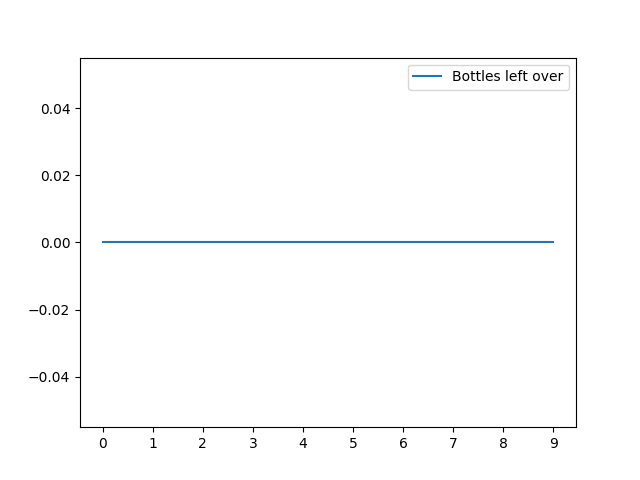
\includegraphics[width=0.49\textwidth]{./python/bots1.png}
    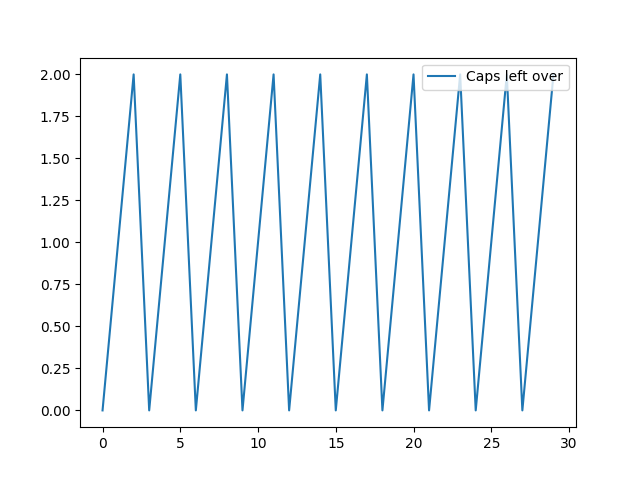
\includegraphics[width=0.49\textwidth]{./python/caps1.png}
\end{center}
From this it makes sense that you'd never end up with a bottle since having one left would always allow you to get another one (boohoo, special case).
The repeating structure of the bottle caps, while not what you may initially think, is not too hard to figure out.
\subsection{Algebraic Solution}
Let $\vec{i}$ be the initial state, $\vec{f}$ be the final state, $c$ be the cap-based transactions, and $b$ be the bottle-based transaction.
\begin{align*}
    \vec{i}
    + c
    \begin{bmatrix}
        -3\\
        1
    \end{bmatrix}
    + b
    \begin{bmatrix}
        1\\
        -1
    \end{bmatrix}
    &=
    \vec{f}\\
    c
    \begin{bmatrix}
        -3\\
        1
    \end{bmatrix}
    + b
    \begin{bmatrix}
        1\\
        -1
    \end{bmatrix}
    &=
    \vec{f} - \vec{i}\\
    \begin{bmatrix}
        -3 & 1\\
         1 &-1
    \end{bmatrix}
    \begin{bmatrix}
        c\\
        b
    \end{bmatrix}
    &=
    \vec{f} - \vec{i}\\
    \begin{bmatrix}
        c\\
        b
    \end{bmatrix}
    &=
    \frac{1}{2}
    \begin{bmatrix}
        -1 &-1\\
        -1 &-3
    \end{bmatrix}
    (\vec{f} - \vec{i})\\
\end{align*}
The goal is to get as drunk as possible, which is reaching as many transactions as possible, thus we want to maximize $b + c$ with respect to the elements of $f$.
\begin{align*}
    c + b &= \frac{1}{2}(-2(f_c - i_c) - 4(f_b - i_b))
    %\frac{\partial(c + b)}{\partial f_c \partial f_b} &= \frac{1}{2}(-2(f_c - i_c) - 4(f_b - i_b))
\end{align*}
Since there's not that many possible combinations of $\vec{f}$, it would be practical in this case to simply check for the maximum, but that's no fun.
\section{Using the final state of the vector to deduce the amount of drinks one had}
\par Since two empty bottles can get you a drink and a drink is worth \$2, then that means one bottle is worth \$1.
Similarly since four bottle caps can get you a drink and a drink is worth \$2, then that means bottle cap is worth \$0.5.
\par Since a full drink is consisted of one cap, one bottle, and some drink, we can use simple algebra to deduce that:
\begin{equation}
    \$2 = d + \$1 + \$0.5
\end{equation}
\begin{equation}
    d = \$0.5
\end{equation}
the worth of the drink is \$0.5.
If we started with \$10 dollars, and we are left with $a$ bottles and $b$ caps, then:
\begin{equation}
    \$10 = \$0.5x + \$a + \$0.5b
\end{equation}
\begin{equation}
    x = \frac{\$10 - \$a - \$0.5b}{\$0.5}
\end{equation}
\end{document}
